\chapter{Approach}

\begin{itemize}
\item define language models
\item Describe problems with common language models
\item define solutions to these problems 
\item show why our model is a solution
\end{itemize}

\newcommand{\NN}{\mathbb{N}}

\paragraph*{Language Models}
The basic operation implemented by any language model is to predict an unknown sequence element given a surrounding context.
\begin{align}
    P(x_{n+1} \mid x_0, \ldots, x_n)
\end{align}

\paragraph*{String-Containment Graph}
A string containment graph $G = (V, E)$ of a string $s$ is the graph of the string-containment relation on substrings of $s$. With the \textbf{substring relation} $x \sqsubset y$ (''$x$ is contained in $y$'') defined as:
\begin{align}
    & \forall (x, y) \in \Sigma^*: x \sqsubset y &\Leftrightarrow& \quad &\exists \ (a, b) \in ({\Sigma^*}^2) \setminus {(\epsilon, \epsilon)}: y = axb
\end{align}
The nodes $V$ are the set of all substrings in $s$:
\begin{align}
    &V := \{ x \in \Sigma^* \mid s = axb, a, b \in \Sigma^*\}
\end{align}
(Note that $s \in V$.)\\
and an edge $(x, y, o) \in E \subseteq (V^2 \times \NN) $ exists iff $x$ is a substring of $y$ at an offset $o$:
\begin{align}
    E := \{ (x, y, o) \mid x \sqsubset y, o = |a| \ \text{where} \ y = axb, x, y \in V \}
\end{align}

\paragraph*{N-Gram Vertex Contexts \& Substrings}
Within a string containment graph we denote the set of (direct) contexts $Ctx(v)$ of a vertex $v$ as the parent set of $v$ in the graph:
\begin{align}
    Ctx(v) := \{ p \in V \mid \exists \ (v, p, o) \in E \}
\end{align}
In the same way the set of (direct) substrings is defined as the child set of $v$ in the graph:
\begin{align}
    Sub(v) := \{ s \in V \mid \exists \ (s, v, o) \in E \}
\end{align}

\newpage
\begin{align}
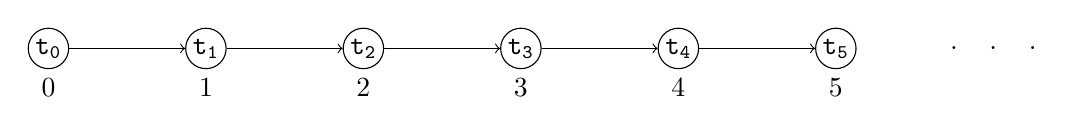
\begin{tikzpicture}
\newcommand\N{5};
\foreach\x in{0, ..., \N}{
    \node[draw,
        circle,
        inner sep = 1pt,
        scale=1.0,
        label=below:\x
    ] (T\x) at (2*\x, 0) {$ \mathtt{t_\x}$};
}
\foreach\x in{1, ..., 3}{
\pgfmathtruncatemacro{\name}{\N + \x};
\node (\name) at ({2*\N + 1 + \x*0.5}, 0) {$.$};
}
\pgfmathtruncatemacro{\ne}{\N - 1};
\foreach\x in{0, ..., \ne}{
    \pgfmathtruncatemacro{\next}{\x + 1};
    \draw [-to](T\x) -- (T\next);
}
%\draw [-to](0) -- (1);
\end{tikzpicture}
\end{align}

\newpage
In this chapter we describe the algorithms for constructing the hierarchical n-gram grammar and applying it as a language model. First we describe the target structure and how it can be used to predict completions for a given sequence, then we describe an algorithm for inducing the structure from a single input string or a set of strings.

\begin{itemize}
    \item \textbf{Induction:} Construct new rules to represent a given string of symbols
    \item \textbf{Search:} Find grammar rules related to a given string of symbols
\end{itemize}

\section{Context Graph Structure}
The basic objective of the structure is to connect each frequent n-gram $x$ to all of its contexts, that is, strictly larger n-grams where $x$ occurs as a substring. 
This structure can be described as a partial order between n-grams, which forms a directed graph where the nodes are n-grams which are connected with a directed edge if the first n-gram contains the second n-gram at any offset.
%The total number of possible contexts grows quadratically with the length $N$ of the root N-gram:
%\begin{align}
%N - n_x
\section{Foundations}
\paragraph{Ambiguous Grammars}

\section{Induction Phase}
% describe reading target
How is the grammar built from a given input string?

\paragraph{Grammar Traversal}
%Essential to using the model is the search of known sequences.
%In this section we will describe how the model can be used to parse an input string,
%effectively searching the model for known information about the string.
This provides us with one example of how the nodes and edges of the graph can be
iteratively visited and worked on.
In principle the parsing stage employs a bottom up, Generalized-Left-Right(GLR)-Parsing 
process, which uses a graph-structured stack (GSS) to traverse all possible parse trees 
of the input.
%\begin{align}
%
%\end{align}

\paragraph{GLR-Parsing}
The algorithm works by walking upwards over all parent nodes of the starting symbol of 
the input.
For each parent, it attempts to compare the remaining input with the remaining input of 
the parent node.
Abstractly, the algorithm will continue to expand nodes upwards until it finds a parent 
with a matching
continuation (or exhausted all known contexts and reports a mismatch).
When a matching continuation is found, all alternative parse trees can be abandoned as 
they all lead either
to different contexts than the smallest unique one, or must lead to the same parent.
(convincing formal proof)
This can be derived from the equal children axiom and the fact that breadth first search 
will search parents
in a width-ascending order.

All sequences known to the model can be found by starting at any symbol and traversing 
its parent contexts in a bottom up iterative process. When given a search query in the 
form of a sequence, we can start with any of the symbols and match the surrounding 
symbols in the query with the contexts stored in the model grammar. This is basically a 
parsing problem where we try to parse a given word of a grammar.

Not all of the symbols in the query need to be atomic symbols. We can match non-atomic symbols the same way we match symbols in model grammar rules. We provide an overview of the algorithm and a more detailed pseudo-code representation below. The result of the parsing process is a rooted sub-graph structure containing the paths traversed during the parsing process, with the smallest symbol containing the entire known sequence as a root. 

\subsection{Construction}

\paragraph{Reusing partitions}
With navigational information from search, an infrequent sequence can be compressed into an identifying symbol. This is needed to compress larger sequences of smaller known sequences.

During search, paths over the grammar are traced and combined to a sub-graph visiting all leaf nodes of a subsequence in a root symbol.

\paragraph{Partitioning Rules}
The sub-graph structure resulting from a search contains all of the information needed to create a new symbol representing the identified sequence. The paths contained in the sub-graph point to the exact locations where the partition intersects rules in the grammar, which we need to modify to support the new symbol about to be added to the index.

The basic idea is to find all of the locations where intersected symbols need to be split into partitions which can then be used to build larger symbols without repeating sequences in any rules (which would violate invariant 3).

\subsection{Counting}
Upper bound for repeated substrings in a string of length $N$ over an alphabet of $k$ symbols:


\subsection{Consuming Sequences}
In order to consume new sequences and add them to the model, we require a set of algorithms on the grammar structure described in the remainder of this section. The process can be divided in three major stages, each working on the results of the previous stage:
\begin{enumerate}
\item Search largest known partition at position
\item Join partition sub-graph into new symbol
\item Join found partitions into new symbol for the entire input sequence
\end{enumerate}

When reading new symbols, we want to construct them in a way that upholds certain properties to make the resulting graph structure space efficient and useful for traversal:
\begin{itemize}
    \item \textbf{Digram Uniqueness} Every string of symbols in all rules in the graph occurs at most once.
    \begin{gather*}
        \forall r_a, r_b \in R, i \in \{ 0, ..., |r_a| - 2 \}, j \in \{ 0, ..., |r_b| - 2 \}:\\
        a \neq b \lor i \neq j \Longrightarrow (r_a[i], r_a[i + 1]) \neq (r_b[j], r_b[j + 1])
    \end{gather*}

    \item \textbf{Deterministic Expansions} Each symbol represents a single string. Every rule of the symbol produces the same string.
    \begin{align*}
        \forall s \in V, r_i, r_j \in R_s: \texttt{expand}_G(r_i) = \texttt{expand}_G(r_j)
    \end{align*}

    \item \textbf{Edge Completeness} Every symbol must contain all largest symbols representing any of its sub-strings in its rules.
    \begin{align*}
        \forall a, s \in V&: \texttt{expand}_G(a) \text{ substring of } \texttt{expand}_G(s) \\
        &\nexists b \in V: \texttt{expand}_G(a) \text{ substring of } \texttt{expand}_G(b) \\
        %%&\land  \texttt{expand}_G(b) \text{ substring of } \texttt{expand}_G(s) \RightArrow \exists r \in s: a \in r
    \end{align*}

    \item \textbf{No Shared Boundaries} All boundaries between two rule symbols in a symbol represent unique positions in the expanded string.
    \begin{gather*}
    \end{gather*}
\end{itemize}

\subsection{Tracing Overlaps}
The goal is to find all largest non-terminals represented in a word, even if they are overlapping and to create
new non-terminals if it is necessary to uphold the minimalism in the resulting production rule.

We can start by parsing the first largest non-terminal from the left to right.
If there are no more tokens in the input word, we have found a single non-terminal
producing the word and we are done. However if there are more tokens we were
not able to parse, we know that we need to create a new production rule for this input word.

We could just continue parsing the next largest symbols and append them into a single rule,
but this would not uphold the property that each set of parallel production rules contains all of the
largest symbols expanding to parts of the produced word. There may be symbols which produce overlapping
sequences of the word and the largest of those need to be included into the new set of production rules.

To find these overlaps as efficiently as possible, we perform a search locally around symbols we have
previously found. This reduces the search space and makes use of previously computed results.

After we have parsed the first largest symbol, we want to find the next largest overlap with this symbol.
So we search top-down through all of the postfixes of the symbol from largest to smallest, and for each
we try to parse the word resulting from appending the postfix with the remaining tokens from the input word.
We either never find a symbol representing any overlap, in which case we simply continue parsing the remaining input,
or we find an overlap. An overlap starts with some postfix from the former symbol, i.e. it
uses it as a prefix in one of its rules. To build the resulting set of production rules, we need to complete the
context in backward direction, to represent the sequence before the overlap. For this we can make use of the parse
tree of the former symbol of which we searched a postfix. By accumulating the backward context along all of the
levels of its parse tree, we can create a new production rule representing the backward context of the overlap. (PROOF)

In the resulting state we have two bands or two production rules, each representing a prefix of the input word of
different lengths. We now continue to search for overlaps of the now latest symbol, i.e. the former overlap we have
just found. Overlaps for this symbol could also overlap with the symbol we were previously finding overlaps for.
However we can disprove that this can be the case if the production rule of the overlapping entry, i.e. the one
starting with the postfix of the previous symbol, contains more than two symbols. This follows from the condition 
that no sequence of symbols may appear twice anywhere in the entire grammar. Only if there is exactly one symbol 
following the former postfix, may that same sequence appear in another larger symbol. We can use this knowledge to 
decide our next steps.

In the case where there are at least two symbols following the first in the rule, we know that any overlaps must begin 
after the end of the last symbol we overlapped. If there is only one following symbol, however, there may be an overlap 
with the current symbol and also the previous symbol. If such a symbol exists, there must be a production rule in the 
current symbol with a postfix larger than that of the rule we entered the current symbol through, because of the 
maximality constraint. We can use this postfix to find the next overlap, however the postfix may not be expandable into 
the following tokens. We search throught the postfixes in descending order. We will eventually encounter the postfix of 
the rule we entered through. We use it to complete the rule with the first symbol we parsed by appending it. If the 
postfix is expandable, we append the extension. This extension is then overlapping with the current symbol and we can 
move on to repeat the algorithm inside the extension.

Earlier, we mentioned the case where the entry rule of a symbol contained more than two symbols, and that in this case 
we know that there can be no overlap with the current symbol starting at or before the end of the last symbol. But there 
can still be an overlap with the current symbol which starts after the end of the last symbol. In case we don't find any 
overlaps, we will simply create a new symbol for the postfix of the current symbol after the entry from the last symbol 
and append it to the band with the last symbol. We get two bands with different rules but generating the same strings 
(which are of equal length). We create a new symbol for these two bands and replace them with it, because we can not have 
two boundaries at the same string position in any rules of one symbol. 

